\documentclass[a4paper,man,natbib,floatsintext,donotrepeattitle]{apa6}
\usepackage[english]{babel}
\usepackage[utf8x]{inputenc}
\usepackage{amsmath}
\usepackage{graphicx}
\usepackage{xcolor}
\usepackage[draft,inline,nomargin,index]{fixme}
\usepackage[hidelinks]{hyperref}
\usepackage{verbatim}
\usepackage{nameref}
\usepackage{lineno}
\usepackage{amsfonts}
\usepackage{booktabs}
\usepackage{siunitx}
\usepackage[symbol]{footmisc}
\usepackage{dirtytalk}

% for comments
\usepackage{todonotes}

% adding an epigraph
\usepackage{epigraph}

% epigraph text size
% \renewcommand{\epigraphsize}{\large}

% changing epigraph width
\setlength{\epigraphwidth}{0.75\textwidth}

% right-align epigraph
\renewcommand{\textflush}{flushright}

% adapting dois to follow APA6
\newcommand*{\doi}[1]{\href{http://dx.doi.org/#1}{ #1}}

% new command for Donny's comments
\newcommand{\DWcomment}[2][inline]{\todo[author=DW, color=red!20, #1]{#2}}

% enabling line numbers
\linenumbers

\title{A parsimonious view on the frequentist vs Bayesian debate, a commentary on \cite{albers_credible_2018}}
\shorttitle{Pragmatism versus parsimony}

\twoauthors{Ladislas Nalborczyk}{Paul-Christian Bürkner}
\twoaffiliations{Univ. Grenoble Alpes, CNRS, LPNC, 38000, Grenoble, France \\ Department of Experimental Clinical and Health Psychology, Ghent University}{Department of Psychology, University of Münster, Germany}

\abstract{Based on the observation that frequentist confidence intervals and Bayesian credible intervals sometimes happen to have the same numerical boundaries (under very specific conditions), \cite{albers_credible_2018} proposed to adopt the heuristic according to which we can usually treat them as \textit{equivalent}. We argue that this is potentially misleading and would add to the existing confusion. We instead advocate for the use of parsimony in deciding which statistics to report. In a word, we recommend that a researcher interested in the Bayesian interpretation simply reports credible intervals along with sensitivity analyses.}

\keywords{Bayes, Bayesian statistics, confidence interval, credible interval}

\authornote{Correspondence concerning this article should be addressed to Ladislas Nalborczyk, Laboratoire de Psychologie et Neurocognition, Univ. Grenoble Alpes, 1251 avenue centrale, 38058 Grenoble Cedex 9, France. E-mail: \href{mailto:ladislas.nalborczyk@gmail.com}{\nolinkurl{ladislas.nalborczyk@gmail.com}}.}

\begin{document}

% defining a new command for counting words
\newcommand{\quickwordcount}{
  \immediate\write18{texcount -1 -sum -merge main.tex > \jobname-words.sum}
  \input{\jobname-words.sum}words
}

\maketitle

Wordcount: This document contains \textbf{\quickwordcount}.

\newpage

% restoring section numbering (disabled by the apa template)
\setcounter{secnumdepth}{2}

\epigraph{If a thing can be done adequately by means of one, it is superfluous to do it by means of several; for we observe that nature does not employ two instruments where one suffices.}{\textit{Aquinas, [BW], p.129}}

\section{Context}

\DWcomment{\textbf{General Comments:} From reading the work, I was thinking it might be a good idea to provide examples of when the intervals are not equivalent. I have an example and can provide it if interested. And about the pragmatic position, I think that one further point is the pragmatism should not take the place of statistical literacy. So really highlighting when they will and will not be the same, even with non-informative priors. Also, I see their position as potentially dangerous, as if using Bayes to see if an interval excludes zero, I would suggest this is doing NHST. However, because it is Bayesian, people might now be aware that error control should be considered, etc. On the other hand, the posterior not only allows for probabilistic statements, but can also be used to compute directional Bayes factors. So maybe an example of this to make it clearer, rather than just stating it.}

\cite{albers_credible_2018} proposed a very clear and concise discussion of the frequentist versus Bayesian debate from a pragmatic perspective, offering refreshing and thought-provoking ideas on this old debate.

The main line of reasoning of \cite{albers_credible_2018} seems to be the following: as frequentist confidence intervals and Bayesian credible intervals give the same numerical boundaries (in most situations according to their reasoning), we can interpret them the same way. More precisely, they argue that because confidence intervals and credible intervals do sometimes have the same numerical boundaries (and because when they do they have similar consequences on the inference being made), then, from a pragmatic perspective, they should be treated as \textit{equivalent}.

% making footnotes in arabic style
\renewcommand{\thefootnote}{\arabic{footnote}}

However, we argue that i) even in the (actually rare) situations where the numerical boundaries of the intervals are identical (mostly in simplistic examples), the inference we make from each interval is not identical, and that ii) pragmatism comes with its own pitfalls, that could easily be avoided by using parsimony instead as a guiding principle.

\section{Rebuttals}

\subsection{Restating Bayes theorem, a tautology}

From a broad perspective, outlining that confidence intervals are usually equivalent to credible intervals when using non-informative priors is akin to simply rephrasing Bayes theorem, which states that the posterior is proportional to the likelihood times the prior, that is:

$$ posterior \propto likelihood \times prior $$

From this theorem, we can deduce that if the prior is non-informative, then the posterior can be equated with the likelihood. It follows that frequentist estimates (who depends only on the likelihood) can be equated with Bayesian estimates (that are obtained from the posterior distribution) when uninformative priors are used. In other words, frequentist statistics can be conceived as a particular case of Bayesian statistics. Given that this conclusion is a strict deduction from Bayes theorem, we feel that rhetorical demonstrations and numerical simulations aiming at demonstrating this equality would add very little to the current state of knowledge. As an analogy, it would be similar to trying to make an extensive comparison of weight and mass in order to demonstrate that they sometimes happen to have the same value (see below).

\subsection{Conditioning on nonsense}

...

\subsection{Numerical identity is not "ontological" identity}

It is usually not enough for two entities to have the same numerical values to conclude that we can interpret them the same way. It is even less sufficient to allow the conclusion that they have the same characteristics. As an analogy, we discuss in this section a comparison of the concepts of mass and weight.

Both measures can sometimes (under particular conditions of gravitational acceleration) give similar numerical estimations of a physical phenomenon. However, even in this situation, they do have very different meanings.

Mass is a measure of the amount of matter an object is made up of (that we can express in kilograms), while weight refers to the force exerted on an object by gravity (expressed in newtons). The relation between weight ($W$), mass ($M$) and gravitational acceleration ($G$) is given by the following equation:

$$ W = M \times G $$

As an example, the weight of an object of 100kgs on Earth is approximately equal to $100 \times 9.8 = 980 \text{N}$. However, the weight of an object of 100kgs on the Moon is approximately equal to $100 \times 1.622 = 162.2\text{N}$.

Let's now consider an environment $E$ in which $G = 1$ (which can be thought as a flat prior in Bayesian terms). In this environment, $W$ is equal to $M$ and a pragmatical agent would conclude that both concepts are identical, because they seem to describe a similar aspect of the world.

However, this numerical equivalence under restricted (and unrealistic) conditions does not warrant ontological equivalence. In other words, using mass as a proxy for weight would lead to identical numerical estimates in a very limited range of situations (actually in precisely one situation, i.e., when $G = 1$), but would lead to different numerical estimations in all the other situations (i.e., the situations in which gravity differs from exactly 1). To put it simply, the belief that $W = M$ would lead to erroneous predictions in every situation except the one where this belief was formed (a concept also known as overfitting).

In a similar way, a frequentist confidence interval is about $p(data|\theta)$ while a Bayesian credible interval is about $p(\theta|data)$. These are two very different things, that can, occasionally, happen to be numerically equivalent.

\subsection{Risk of overgeneralising}

As discussed in the previous section, \cite{albers_credible_2018} focused on very simplistic situations (the estimation of the mean of an unimodal distribution and the estimation of a proportion) to illustrate their point, without considering the generalisability of the claim. Similarly to the person living in the environment with $G = 1$, we are afraid that the heuristic according to which confidence intervals can be interpreted as credible intervals will lead to disappointment in most situations.

The authors of the target paper should also consider the risk that this paper becomes a reference for justifying the Bayesian interpretation of confidence intervals in situations that do not warrant this interpretation \citep[cf. various examples in][]{morey_fallacy_2015}.

\subsection{Differences matter}

\cite{albers_credible_2018} write: "In the present paper, we have demonstrated by means of various examples that confidence intervals and credible intervals, in various practical situations, are very similar and will lead to the same conclusions for many practical purposes when relatively uninformative priors are used".

Contrary to what the authors postulate, differences between confidence intervals and credible intervals are observable in an incredible large variety of situations (actually, all but one). For instance, i) when samples are small, ii) when the space of the outcome is multi-modal or non-continuous, iii) when the range of data is restricted, and iv) when the prior is at least weakly informative (the first and last points are not specific to intervals).

Combining these four possibilities, we argue that confidence intervals and credible interval actually almost never give similar results. Additionally, and as we previously demonstrated, numerical estimates can be similar, but it does not entail that the conclusion we can draw from it (i.e., the inference being made) should be similar.

In the previous sections, we discussed why we think the logic of the argument presented in \cite{albers_credible_2018} can be misleading. In the following, we suggest an alternative to pragmatism which does not preclude statistical literacy.

%\subsection{Drawbacks of extreme pragmatism}

%In this section, we want to highlight what appears to us as a fallacious argument\footnote{We recognise that the fallacy comes from the imperfect correspondence between confidence intervals and credible intervals.}. As a reminder, \cite{albers_credible_2018} argue that because confidence intervals and credible intervals do sometimes have the same numerical values (and because when they do they have similar consequences on the inference being made), then, from a pragmatic perspective, they should be treated as \textit{equivalent}. Thus, we could use confidence intervals instead of (or in addition to) credible intervals.

%This argument seems to be of the following form: "Because $A$ can sometimes be interpreted as $B$, then we should use $A$ instead of (or in addition to) $B$". Does it mean that if astrology sometimes gives the same results as personality tests, we should use astrology instead of (or in addition to) personality tests ?

\section{Our proposal: ontological simplicity and parsimony}

\subsection{Applying parsimony in scientific and statistical practise}

\cite{albers_credible_2018} write: "By recognizing the near-equivalence between Bayesian and frequentist estimation intervals in ‘regular cases’, one can benefit from both worlds by incorporating both types of analysis in their study, which will lead to additional insights."

Confidences intervals are a particular case of credible intervals for which priors are non informative. Thus, one could ask, in consideration of the parsimony principle, why reporting redundant statistics ? Why bother to use the particular (i.e., more restricted in its use) case ? Would not it be easier to use the more general and flexible case ? The parsimonious stance that we adopt here lead to the conclusion that the researcher interested in one specific interpretation should report the statistics that corresponds to this goal\footnote{Obviously it is legitimate to be interested in several goals, but in this case, these goals should be clearly stated as separated goals, that we pursue using appropriate tools.}. If a researcher is interested in the sampling distribution of the statistics under study, s$\cdot$he should probably report confidence intervals. If s$\cdot$he is rather interested in making conditional probability statements from the data, then s$\cdot$he probably should report credible intervals.

\subsection{Frequentist characteristics of Bayesian credible intervals}

In Figure \ref{fig:coverage}, we present some simulation results showing that Bayesian credible intervals (obtained with flat priors) do have the same properties as frequentist confidence intervals. Indeed, on repeated sampling, X\% of the constructed intervals will contain the population value of $\theta$.

\begin{figure}[H]
  \caption{Coverage properties of Bayesian credible intervals when using weakly informative priors.}
  \centering
  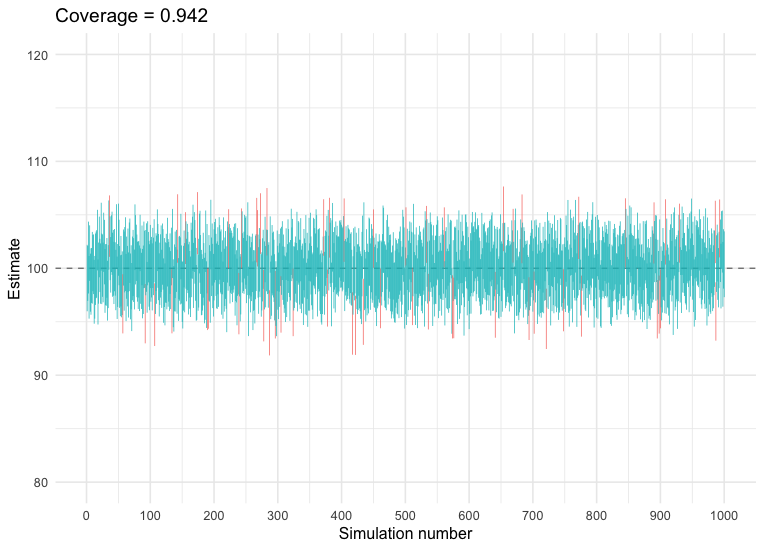
\includegraphics[width=0.8\textwidth]{coverage.png}
  \label{fig:coverage}
\end{figure}

Bayesian credible intervals with non-informative or weakly informative priors do have the same frequentist characteristics as confidence intervals, but also allow conditional probability statements (e.g., given the prior and the information contained in the data, there is a X\% probability that the population value of $\theta$ lies in the interval).

Therefore, the principle of parsimony would lead to use and report the most inclusive (general) statistics. In contrast to what \cite{albers_credible_2018} advocate, we thus suggest that the researcher interested in the Bayesian interpretation should use and report Bayesian statistics along with sensitivity analyses, with both non-informative, weakly-informative or informative priors.

\subsection{A short note on the frequentist properties of Bayesian procedures}

\cite{albers_credible_2018} quote \cite{bayarri_interplay_2004} that wrote: "Statisticians should readily use both Bayesian and frequentist ideas".

We could not agree more with this statement (cf. previous section). In addition, we recognise that both statistical traditions have their own advantages and drawbacks, and have been built to answer somehow different questions. Therefore, we feel that pretending that a statistic issued from one school of inference can be interpreted as a statistic issued from another school because they sometimes (under very restricted conditions) give the same numerical estimates is confusing and potentially misleading.

\section{Conclusions and practical recommendations}

We suggest parsimony as a guiding principle for practical use of frequentist versus Bayesian statistics (see section 3.1), given the limitations of the pragmatic perspective offered by \cite{albers_credible_2018} (see section 2.2 and 2.3), and its potential harmful consequences (see sections 2.4 and 2.5).

In order to warrant the Bayesian interpretation of frequentist confidence intervals, each confidence interval should be accompanied by a Bayesian credible interval. However, as shown by \cite{albers_credible_2018} and by the simulation results we reported in section 3.2, this would lead to redundant intervals, when non-informative priors are used. For the sake of parsimony, we therefore recommend that a researcher interested in the Bayesian interpretation of an interval simply report credible intervals along with sensitivity analyses.

As put by \cite{morey_fallacy_2015}, "More broadly, the defense of confidence procedures by noting that, in some restricted cases, they numerically correspond to Bayesian procedures is actually no defense at all."

\section{Acknowledgements}

...

\bibliography{parsimony}

\end{document}
